\section{Isomorphisme cannonique de McKay}

\begin{frame}{Idée 3 : Isomorphisme cannonique de McKay}
\begin{tabular}{ll}
\underline{Idée générale}: & $\bullet \quad$ tri équitable des sommets à partir d'un tri \\
& $\quad \rightarrow \quad$ informations avec la propagation du degré \\
& $\quad \rightarrow \quad$ tri optimal \\
& \\
& $\bullet \quad$ création d'un arbre de recherche de permutations \\
& $\quad \rightarrow \quad$ on crée artificiellement de nouveux tris équitables \\
& $\qquad \quad$ (fils de l'arbre) en isolant des sommets \\
& $\quad \rightarrow \quad$ les feuilles sont des tris ordonnés de parties à un \\ 
& $\qquad \quad$ sommet : ce sont des permutations \\
& $\bullet \quad$ définition d'un ordre total sur les graphes \\
& $\quad \rightarrow \quad$ déterminer le plus grand pour cette relation parmi \\
& $\qquad \quad$ les graphes permutés avec les feuilles de l'arbre \\
& $\quad \rightarrow \quad$ on obtient alors l'\underline{isomorphisme cannonique}
\end{tabular}
\end{frame}

\subsection{Tri équitable}
\begin{frame}{Tri des sommets encore plus fin}
    \begin{center}
        \underline{Utilisation de la propagation du degré} :
    \end{center}
    Tri des sommets des paquets par degré dans les autres paquets pour en faire un nouveau tri \newline
    $\quad \rightarrow \ $ jusqu'à ce qu'il n'y ait plus de simplifications possibles \newline \newline
    \underline{Exemple} :
    \begin{align*}
        \text{Soit } \pi &= (1\ |\ 3\ 7\ 9\ |\ 6\ 8\ |\ 2\ 4\ |\ 5) \text{ un tri des sommets du graphe G} \\
        &= (V_1\ |\ V_2\ |\ V_3 \ | \ V_4\ |\ V_5)
    \end{align*} 
    \begin{minipage}{0.3\textwidth}
        \begin{figure}
        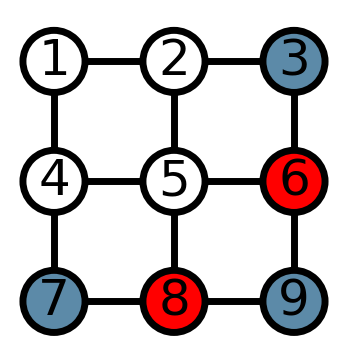
\includegraphics[width = 3cm]{graph_tri_equal_colored} 
        \caption{\label{fig:graphe_tri_equal}Graphe G}
        \end{figure}
    \end{minipage}
    \begin{minipage}{0.25\textwidth}
        \begin{align*}
            \textcolor{airforceblue}{V_2} & \textcolor{airforceblue}{=(3 \ 7\ 9)} \\
            \textcolor{red}{V_3}  & \textcolor{red}{=(6\ 8)}
        \end{align*}
    \end{minipage} 
    \begin{minipage}{0.4\textwidth}
        \begin{align*}
        & \text{Tri de } V_2 \text{ par degré dans } V_3 : \\ \\
        & deg(3,V_3)=deg(7,V_3)=1 \\
        & deg(9,V_3)=2 \\
        & \text{donc } V_2 = (3\ 7\ |\ 9)
        \end{align*}
        \begin{center}
            $\pi ' = (1\ |\ 3\ 7\ |\ 9\ |\ 6\ 8\ |\ 2\ 4\ |\ 5)$
        \end{center}
    \end{minipage}
    \begin{center}
    tri $\pi'$ plus fin
    \end{center}
\end{frame}

\begin{frame}{Tri des sommets encore plus fin : tri équitable}
    \underline{Tri équitable} : la propagation de degré ne donne plus de nouveau tri
    \begin{align*}
        & \forall (i,j)\in[\![1,n]\!]^2, \text{ tous les sommets de } V_i \text{ ont le même degré dans } V_j \\
        \iff \ & \forall (i,j)\in[\![1,n]\!]^2,\ 
        \forall (v,w) \in V_i^2,\ deg(v,V_j)=deg(w,V_j) \\
    \end{align*}
    Soit $\pi$ un tri, on note :
    \begin{equation}
        \boxed{R(\pi) \text{ le plus grand} \footnote{défini selon un ordre partiel sur les partitions}
        \text{ tri équitable ordonné obtenu à partir de \pi}}
    \end{equation} 

\end{frame}

\subsection{Arbre de recherche}
\begin{frame}{Arbre de recherche de permutations}
    \begin{minipage}{0.3\textwidth}
        \begin{figure}[!htb]
            \centering
            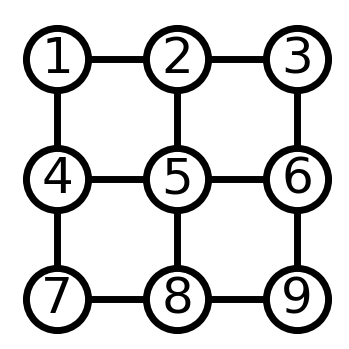
\includegraphics[width = 1.7cm]{graph_tri_equal}
            \caption{\label{fig: Graph G2}Graph G}
        \end{figure}
    \end{minipage}
    \begin{minipage}{0.6\textwidth}
        \begin{center}
            On considère le tri suivant le degré :\newline
            $\pi = (1\ 3\ 7\ 9\ |\ 2\ 4\ 6\ 8\ |\ 5)\qquad $ \newline \newline
            $R(\pi)=\pi$ est alors la racine de l'arbre
        \end{center}
    \end{minipage}
    \newline \newline \newline
    \underline{Trouver les fils} :
    \begin{itemize}
        \item trouver la première partie $V_i$ d'au moins 2 éléments de $\pi$
        \item pour $v \in V$, on crée \textbf{artificiellement} un nouveau tri équitable :
        $\quad \longrightarrow \quad \pi_v = \pi \perp v = R(\ (V_1|..|\ \lbrace v \rbrace \ |\ V_i \textbackslash \lbrace v \rbrace\ |..)\ )$
        \item chacun des tris créés est un fils, on réitère jusqu'à obtenir des tris triviaux (paquets de taille 1)
    \end{itemize}
\end{frame}

\begin{frame}{Arbre de recherche de permutations}
    \begin{figure}[!htb]
        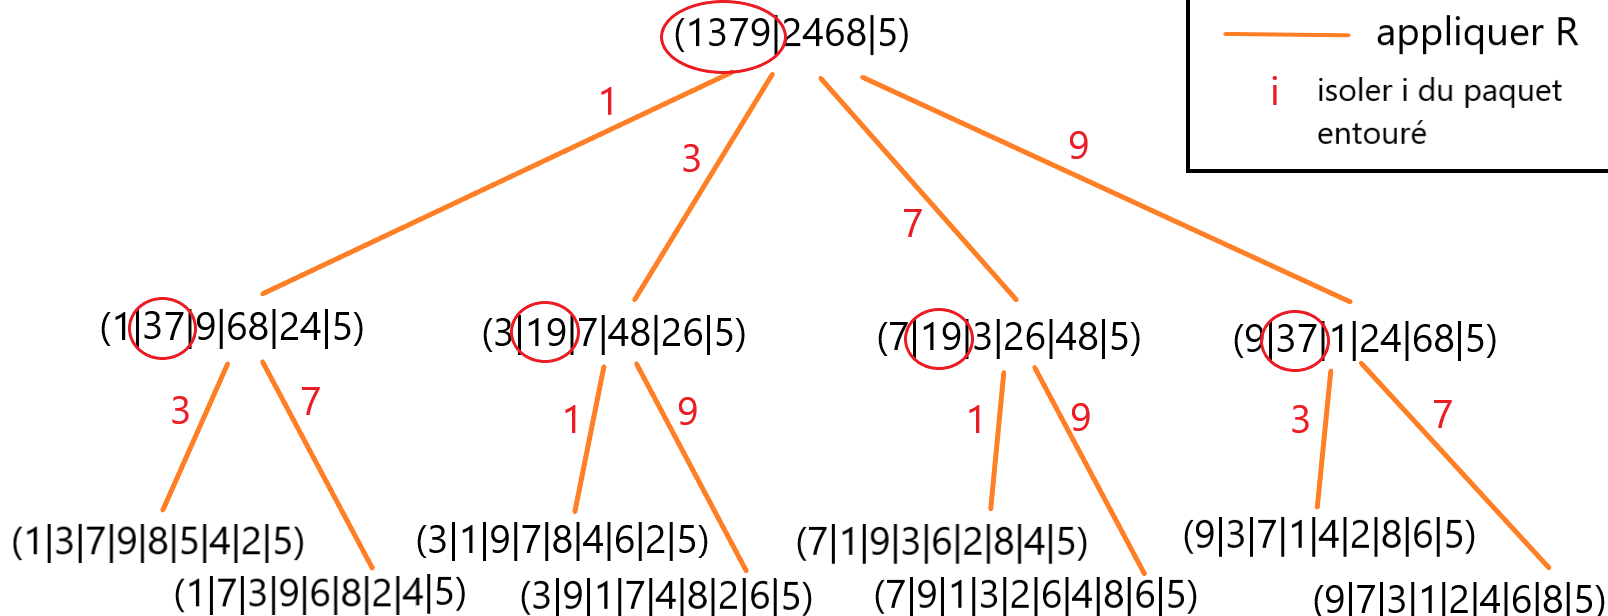
\includegraphics[width = 10cm]{search_tree}
        \caption{\label{fig:Arbre T(G)} Arbre T(G) de racine $\pi=(1\ 3\ 7\ 9\ |\ 2\ 4\ 6\ 8\ |\ 5)$}
    \end{figure}
\end{frame}

\subsection{Isomorphisme cannonique}
\begin{frame}{Relation d'ordre sur les graphes et isomorphisme cannonique}
    \underline{Ordre total $\preceq$ sur les graphes} : \newline \newline
    On pose la fonction $i:\ G\ \longmapsto i(G)$ telle que : \newline
    $\quad \bullet \ i(G)$ est la séquence binaire $(\mathds{1}_{(i,j)\in G})$ dans l'ordre lexicographique \newline
    $\quad \bullet \ G \preceq H$ si et seulement si $i(G) \leq i(H)$ en décimal
    \newline \newline
    On pose alors l'\textbf{ismorphisme cannonique de McKay} (pour le tri $\pi$):
    \begin{equation}
        \boxed{C_M(G) = max_{\preceq}\ \lbrace G^{\sigma},\ \sigma \text{ noeud terminal de T(G) de racine } \pi \rbrace }
    \end{equation}
    alors:
    \begin{equation}
        \boxed{G \cong H \text{ si et seulement si } C_M(G) = C_M(H)}
    \end{equation}
    \newline
    \underline{Exemple} : pour $\pi = (1\ |\ 3\ 7\ |\ 9\ |\ 6\ 8\ |\ 2\ 4\ |\ 5)$
    \begin{multicols}{2}
        \begin{figure}[!htb]
            \centering
            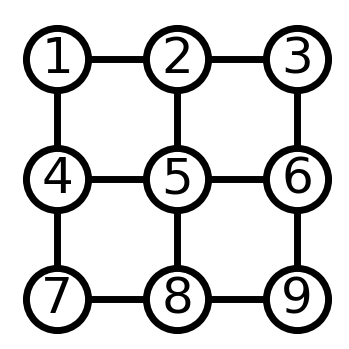
\includegraphics[width = 2.5cm]{graph_tri_equal}
            \caption{\label{fig: Graphe G}Graphe G}
        \end{figure}
        \vspace*{1cm}
        \begin{figure}[!htb]
            \centering
            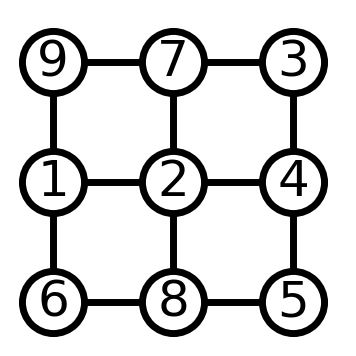
\includegraphics[width = 2.5cm]{cmg}
            \caption{\label{fig: Isomorphe G} Graphe $C_M(G)$}
        \end{figure}
    \end{multicols}
\end{frame}

\subsection{Application}
\begin{frame}{Application sur les protéines}
    \begin{multicols}{2}
        \begin{figure}[!htb]
            \centering
            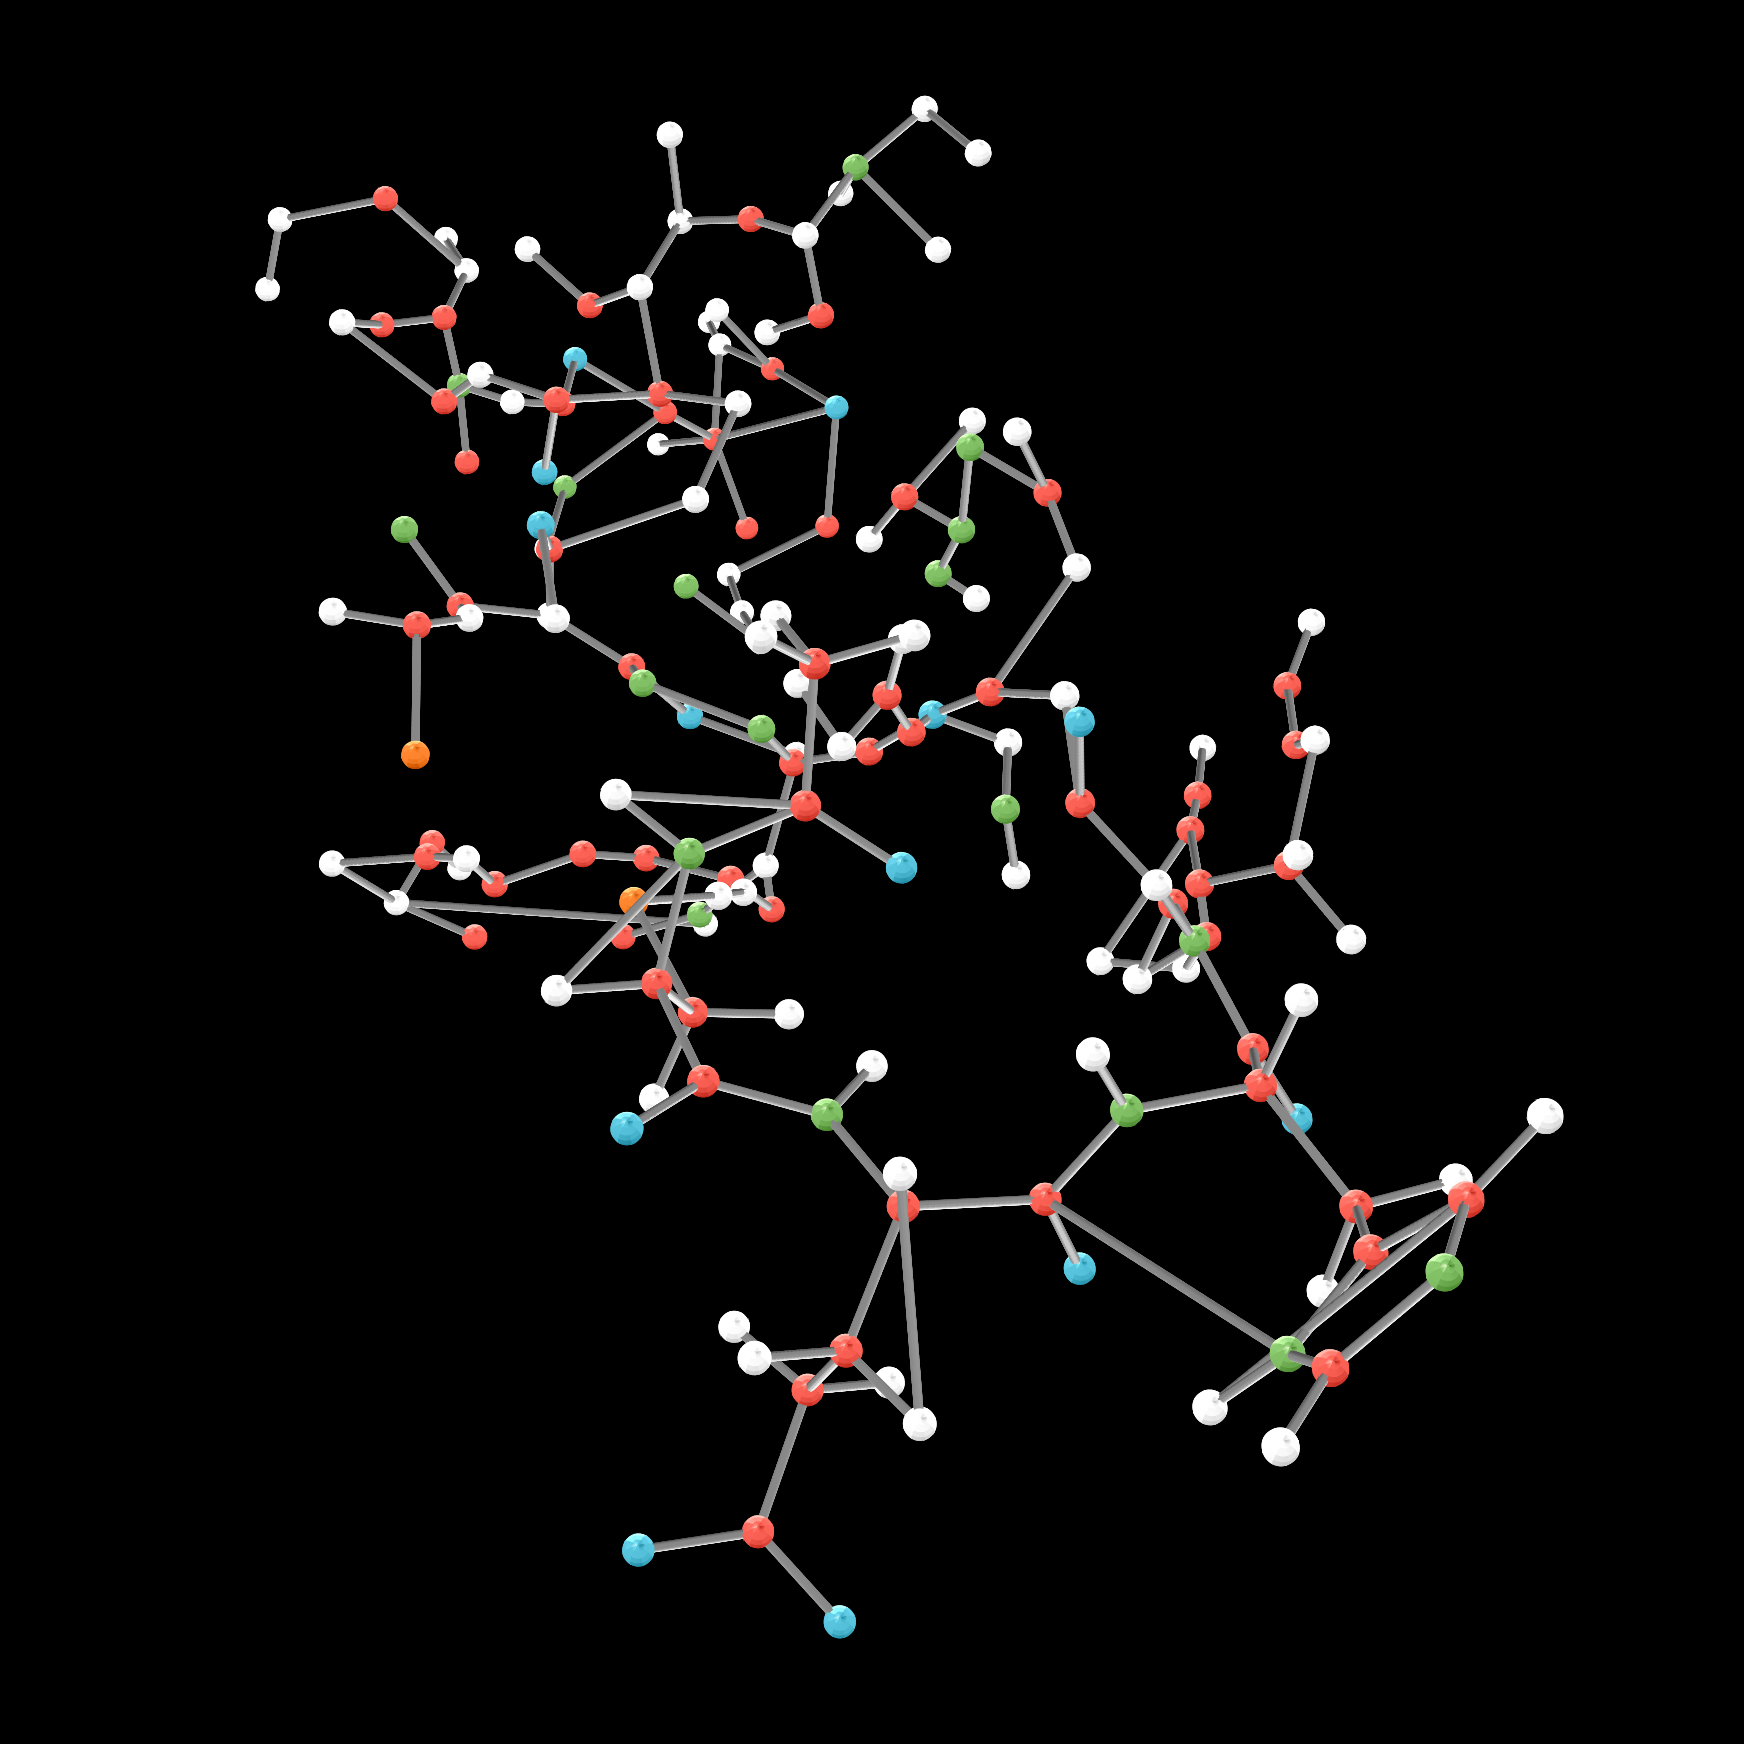
\includegraphics[width = 3cm]{protein_cov}
            \caption{\label{fig: Protéine}Protéine}
        \end{figure}
        \begin{center}
        \begin{figure}[!htb]
            \centering
            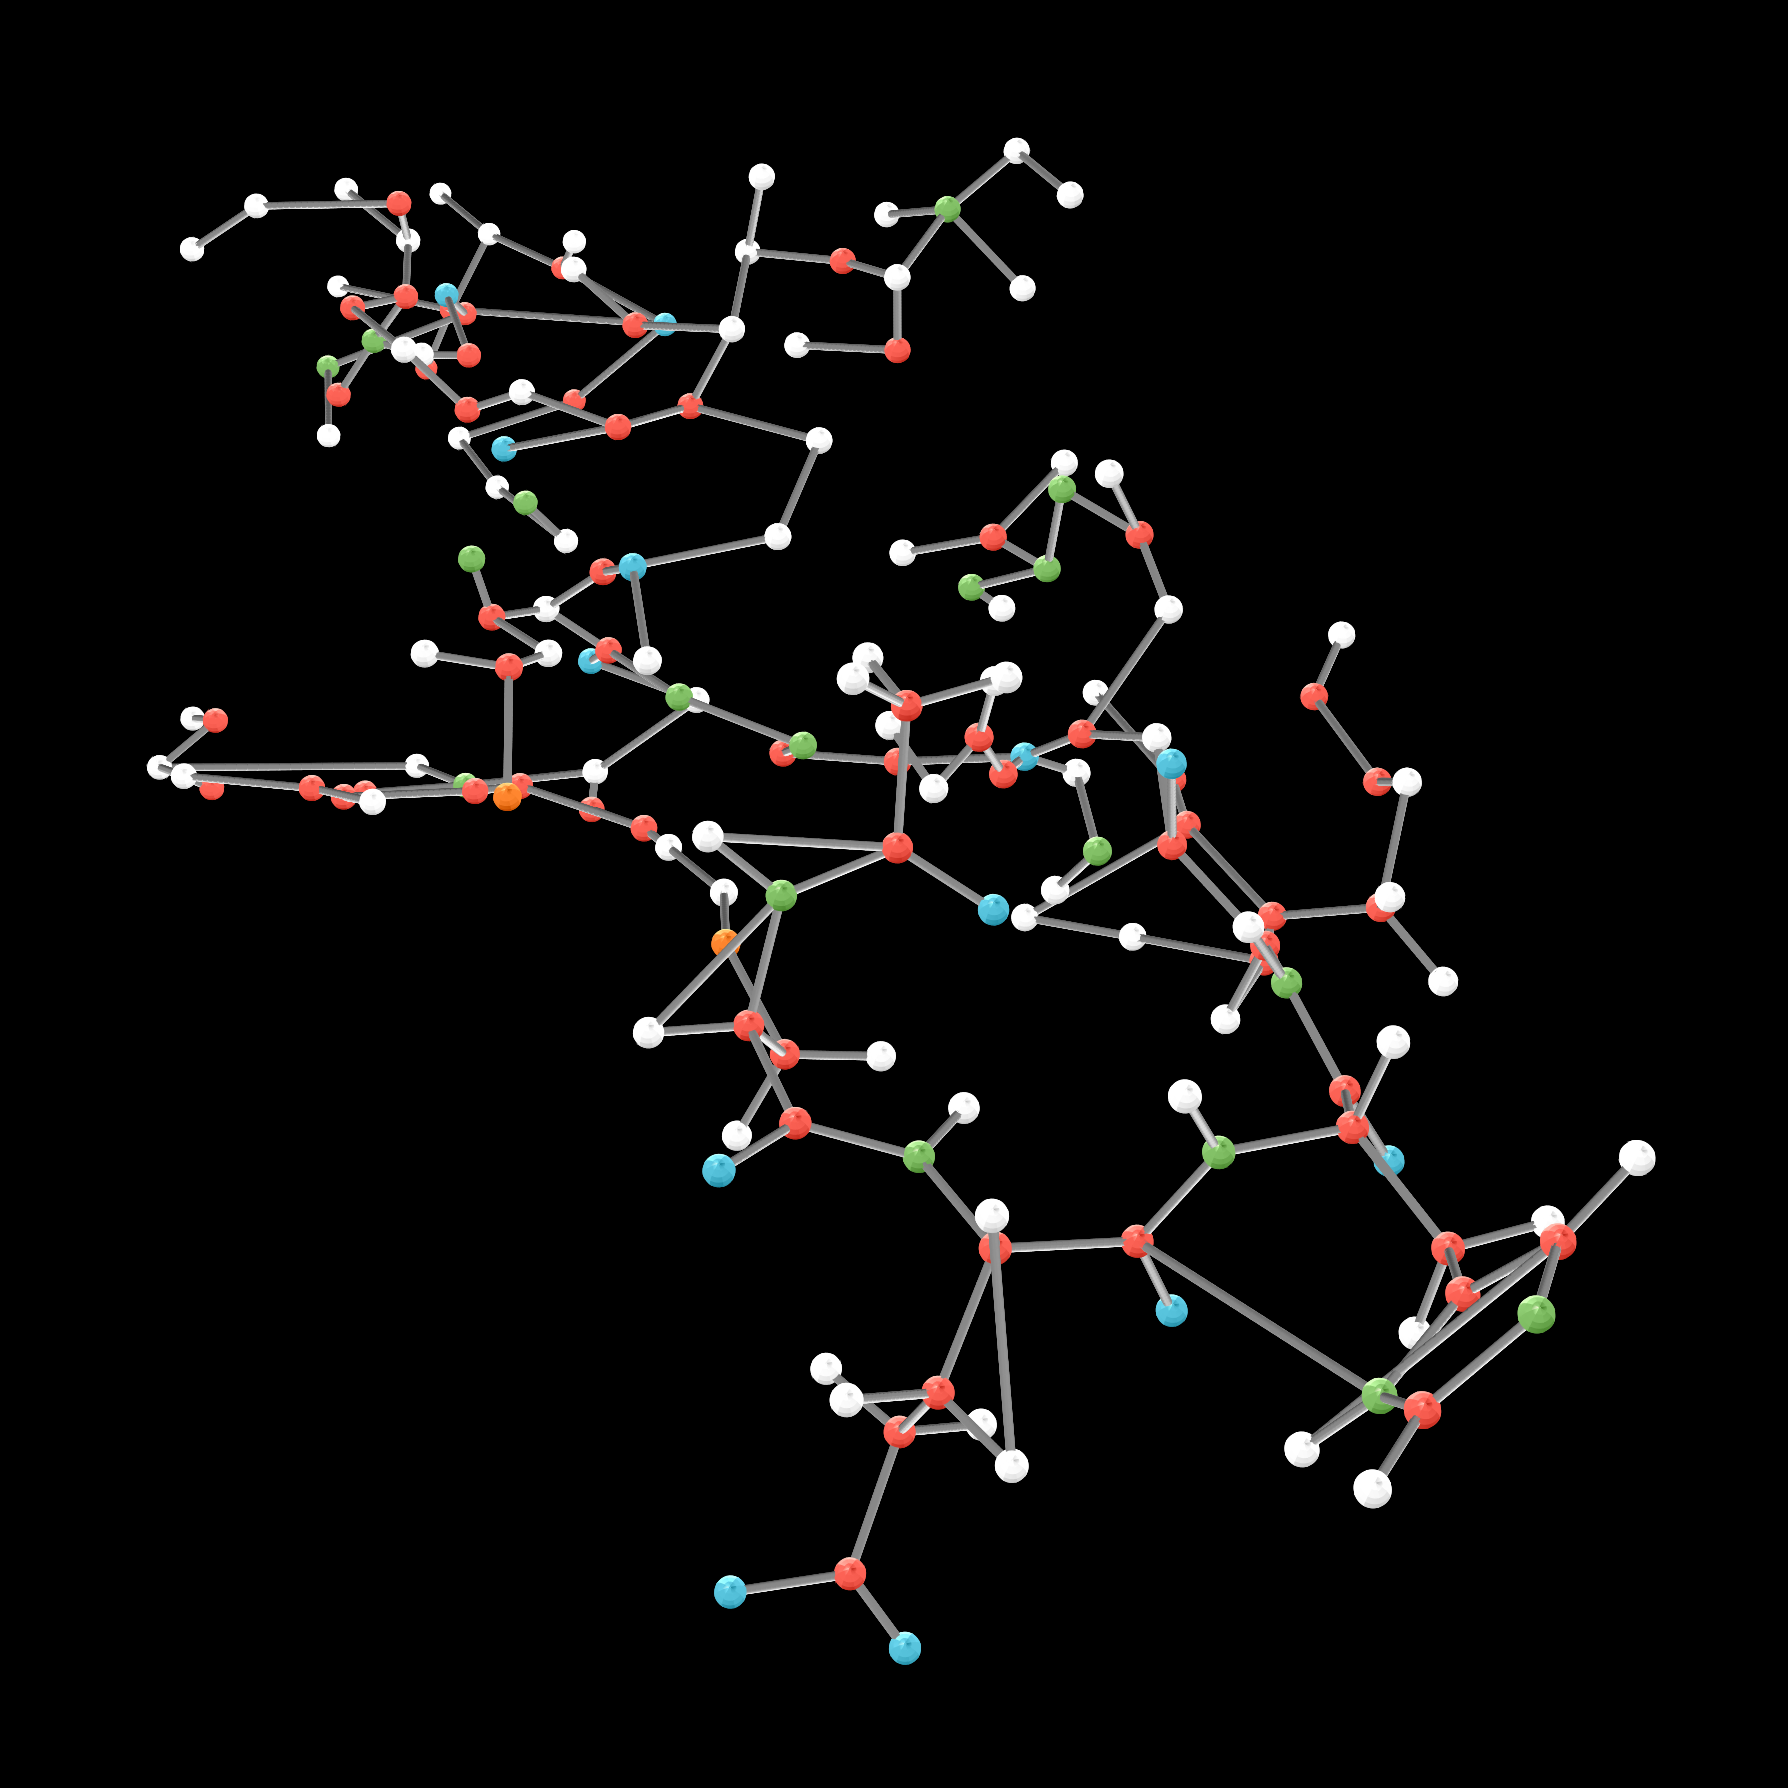
\includegraphics[width = 3cm]{protein_cov_translatee}
            \caption{\label{fig: Protéine translatée}Même protéine mais déplacée et numérotation différente des sommets}
        \end{figure}
    \end{center}
    \end{multicols}
    \underline{Temps d'éxecution} : pour cette protéine de 171 atomes
    \begin{center}
    \begin{tabular}{c|c}
        tri par degré et atomes & 0.002 s\\
        propagation des degrés & 7.4 s \\
        test d'isomorphisme & 0.3 s \\
        temps total d'éxecution & 7.8 s
    \end{tabular}
    \end{center}
    \underline{Résultat} : protéines isomorphes et permutation renvoyée correcte
    \newline tri + propagation du degré $\rightarrow$ paquets d'au plus 4 atomes
\end{frame}